% ==============================================================================
% LAB 118
% GRUNDLÄGGNADE MÄTINSTUMENT
% --------------------------
% Last updated <2015-02-18> 
%
% Author:
% Jonas Sjöberg     <tel12jsg@student.hig.se>
% Oscar Wallberg    <tco13owg@student.hig.se>
% 
% License:
% Creative Commons Attribution-NonCommercial-ShareAlike 4.0 International
% See LICENSE.md for full licensing information.
% ==============================================================================

% ==============================================================================
% INCLUDES AND CONFIGURATION
% ==============================================================================
\documentclass[11pt,a4paper]{article}
\usepackage[utf8]{inputenc}
\usepackage{siunitx} % Provides the \SI{}{} and \si{} command for typesetting SI
\usepackage{amssymb}
\usepackage{amsmath}
\usepackage{amsfonts}
\usepackage{graphicx}
\usepackage{booktabs}
\usepackage{longtable} % Tables span across pages
\usepackage{microtype}
%\usepackage[swedish]{isodate}
\usepackage{gensymb}
%\usepackage{tabto}
\usepackage{units}
\usepackage{siunitx}
  
\setlength\parindent{0pt} % Removes all indentation from paragraphs

% ==============================================================================
% DOCUMENT METADATA 
% ==============================================================================
\title{EE466 \\ Lab 118 \\ Grundläggande Mätinstrument}

\author{\\
  Jonas Sjöberg\\
  Högskolan i Gävle,\\
  Elektronikingenjörsprogrammet,\\
  \texttt{tel12jsg@student.hig.se}\\
  \\
  Oscar Wallberg\\
  Högskolan i Gävle,\\
  Dataingenjörsprogrammet,\\
  \texttt{tco13owg@student.hig.se}\\}

\date{}
% ==============================================================================
\begin{document}
% ==============================================================================
\maketitle

\begin{center}
\begin{tabular}{l r}
    % TODO
    Labb utförd: & DD Month Year \\
    Instruktör: & John Doe, John Doe
\end{tabular}
\end{center}

% ==============================================================================
% ABSTRACT
% ==============================================================================
\begin{abstract}
    Syftet med laborationen är att lära känna de vanligaste basinstrumenten i
    ett elektroniklaboratorium och innefattar övningar i att hantera
    oscilloskop, multimeter, nätaggregat, och funktionsgenerator.
\end{abstract}

\newpage

{
    %\hypersetup{linkcolor=black}
    \setcounter{tocdepth}{3}
    \tableofcontents
}

\newpage

% ==============================================================================
% SECTION: INTRODUKTION 
% ==============================================================================
\section{Introduktion}\label{setup}
% ==============================================================================
Laborationen handlar om olika typer av elektronikinstrument:\\
\begin{tabular}{ll}
\rule{0pt}{3ex}\textbf{Nätaggregat:} & HP 3631A\\
\textbf{Multimeter:} & HP 34401A\\
\textbf{Funktionsgenerator:} & HP 33120A\\
\textbf{Oscilloskop:} & Agilent 54621A
\end{tabular}
\\
\\
I laborationsdokumentet som studerades inför momentet så bifogades korta beskrivningar av instrumenten så att laborenterna kunde bekanta sig med utrustningen i laboreringssalen.\\
\par Med denna kunskap så var uppgiften först att göra mätningar med oscilloskopet, dels över likspänning men även över växelspänning. Fördelen med ett oscilloskop är att användaren kan få grafiska bilder över de intressanta signalerna. \par Den andra uppgiften var att göra mätningar med en multimeter. Fördelen med en multimeter är möjligheterna till matematiska funktioner samt dess noggrannhet med 7 värdesiffror, varav att den första då bara antar värdena 0 eller 1.
% ==============================================================================
% SECTION: 1.1 OSCILLOSKOPET
% ==============================================================================
\section{Oscilloskopet}\label{}
% ==============================================================================
Första uppgiften med oscilloskopet är att mäta spänningen från nätaggregatet tillsammans med multimetmern. Nätaggregatets \unit[6]{\si{\volt}} utgång används och strömgränsen sätts till \unit[0,1]{\si{\ampere}}. Oscilloskopets CH1-ingång ställs till DC-läge och ansluts parallellt med multimetern till nätaggregatet. Multimeterns ``COM'' kopplas till minuspol på nätaggregatet och ``\unit{\si{\volt}}$\Omega$'' till pluspol. Skalfaktorn på oscilloskopet ställs in till \unit[1]{\nicefrac{\si{\volt}}{div}} och multimetern ställs in till likspänning. \par Sedan skall några olika spänningar på nätaggregatet ställas in och både oscilloskopet och multimetern avläses. Skalfaktorn och noll-läget ändras på oscilloskopet för att få en bättre upplösning.
\\
\par Den andra uppgiften är att mäta växelspänningar med oscilloskopet; den ansluts till signalgeneratorn som ställs in på \unit[1]{\si{\kilo\hertz}} sinusvåg med en tidbas på \unit[500]{\nicefrac{\si{\micro\second}}{div}} och en skalfaktor på \unit[1]{\nicefrac{\si{\volt}}{div}}. ``Amplitude'' skall justeras på signalgeneratorn så att en lagomt stor och tydlig bild fås. ``DC offset'' samt ``Symmetry'' skall vara inaktiverade, alltså i detta fall i mittläge. Sedan ändras signalgeneratorns frekvens och man följer efter med oscilloskopets tidbasgenerator. ``Autoscale'' används för att behålla en tydlig bild.
\par Knappen ``Quick meas'' aktiverar oscilloskopets mätfunktion och med ``Soft keys'' (Select -\textgreater Frec -\textgreater Measure) mäts frekvensen. Mätning av andra para\-metrar, t.ex. Amplitude, Pk-Pk, Max, Min och Period, ställs in på samma vis. Några andra kurvformer studeras tillsammans med olika frekvenser och de angivna frekvenserna jämförs med de uppmätta på oscilloskopsbilden.
\par ``DC-offset'' ändras till AC, för att sedan studera skillnaden. Samma signal kopplas till CH2 så att två bilder syns samtidigt. 

\subsection{Mätning av likspänning}\label{meas_dc}
% ------------------------------------------------------------------------------
% TODO

\subsection{Mätning av växelspänning}\label{meas_ac}
% ------------------------------------------------------------------------------
% TODO

% ==============================================================================
% SECTION: MULTIMETERN
% ==============================================================================
\section{Multimetern}\label{}
% ==============================================================================
Vi skall koppla upp en spänningsdelare med två motstånd enligt 
Figur~\ref{fig:2-mm-schem} och använda två multimetrar för att mäta strömmen 
\textbf{I} och spänningen \textbf{U}. Som spänningskälla använder vi 
nätaggregatet. Vi börjar med att välja ut motstånden \textbf{R1} och \textbf{R2}
och undersöka dessa.

\begin{figure}[htbp]
    \centering
        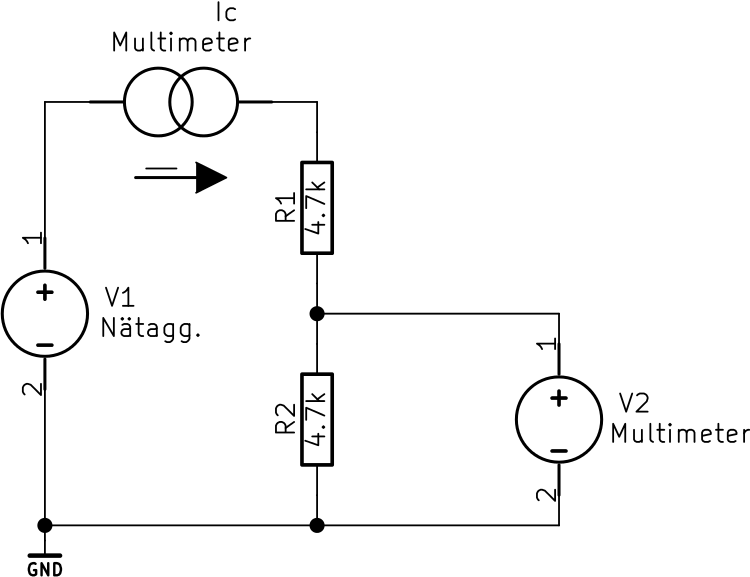
\includegraphics[scale=0.5]{kicad/2-multimeter-schema.png}
    \caption{Spänningsdelarkoppling}
    \label{fig:2-mm-schem}
\end{figure}

Tag två motstånd med olika resistansvärden i området $1-10k\Omega$.
Anslut motstånden till en multimeter med labsladdar och krokodilklämmor.
Mät upp resistanserna med multimetern och jämför med resistansvärdena som är
angivna med färgkoden på motstånden. Välj mätområde på multimetern så att
största antalet siffror (högsta noggrannhet) erhålls.

\begin{longtable}[c]{@{}lll@{}}
    \toprule\addlinespace
    $U_{}$ (V) & Beräknat värde ($\Omega$) &  Uppmätt värde ($\Omega$)
    \\\addlinespace
    \midrule\endhead
    0 & 0 & 0
    \\\addlinespace
    0 & 0 & 0
    \\\addlinespace
    0 & 0 & 0
    \\\addlinespace
    \bottomrule
    \addlinespace
    \caption{Idealfall och mätresultat}
    \label{vdivtable}
\end{longtable}




\subsection{Mätning av spänning, ström och resistans}\label{meas_multi}
% ------------------------------------------------------------------------------
% TODO

\subsection{Mätresultat}\label{TODO}
% ------------------------------------------------------------------------------
% TODO

% ==============================================================================
% SECTION: RESULTAT
% ==============================================================================
\section{Resultat}\label{setup}
% ==============================================================================
% TODO

\newpage

% ==============================================================================
% SECTION: REFERENSER
% ==============================================================================
\section{Referenser}\label{refs}
% ==============================================================================

\subsection{www}\label{interwebs}
% ------------------------------------------------------------------------------
% TODO

\subsection{Trycksaker}\label{literature} %???
% ------------------------------------------------------------------------------
% TODO

%\subsection{Källkod}\label{sourcefiles}
% ------------------------------------------------------------------------------

% ==============================================================================
\end{document}
% ==============================================================================
